% This is the chapter 'Modeling' to the "Hodgkin-Huxley neuron model V2.0 book"
% Last edited 2026.08.10

\ifx\magyar\undefined
\chapter[Elastic model]{Elastic model\label{ch:V2Model-Elastic}}
\else
\chapter[Rugalmas modell]{Rugalmas modell\label{ch:V2Model-Elastic}}
\fi

\iflatexml
\else
\minitoc
\fi

\ifx\magyar\undefined
\quotationbox
{
"Brain cells communicate
with mechanical pulses, not electrical signals" ~\cite{MechanicalBrainPulses:2018}
}
\else
\quotationbox
{
"Az agy sejtjei nem elektromos, hanem mechanikus
impulzusokkal kommunikálnak" ~\cite{MechanicalBrainPulses:2018}
}
\fi

\ifx\magyar\undefined
We introduced the neuron as a lipid ball filled with an aqueous solution, which performs a damped oscillatory motion in a transient state and of course also vibrates the aqueous solution inside. In our model, in a container with a flexible base, a vibration is initiated by a force impact on the base,
which quickly damps down. This model itself belongs purely to the discipline of mechanics. In the case of the neuron, the aqueous solution
contains
ions, and the small amount of ions in the vibrating liquid also performs an oscillatory motion, i.e. generates a voltage wave,
although due to the ions moving back and forth, it only involves minimal material transport.

The mechanical (elastic) model takes us one step closer to the correct model: it is a forerunner of the unified model. It assumes that the action potential is basically generated by the shock wave generated by the elastic membrane, which is significantly distorted by the electrostatic repulsion of the ions in the electrolyte.

\else
A neuront úgy vezettük be, hogy az egy vizes oldattal töltött
lipid gömböcske, ami tranziens állapotban csillapított rezgőmozgást végez, és természetesen a benne található vizes 
oldatot is rezgeti. Modellünkben egy rugalmas alaplappal ellátott
tartályban az alapra ható erőlökéssel rezgést indítunk el,
ami gyorsan lecsillapodik. Önmagában ez a modell tisztán a mechanika 
diszciplinájához tartozik. A neuron esetében a vizes oldat
ionokat tartalmaz, és a vibráló folyadékban levő kis mennyiségű
ion is rezgőmozgást végez, azaz feszültséghullámot generál,
bár az oda-vissza mozgó ionok miatt csupán minimális anyagtranszporttal jár.

A mechenikus (rugalmas) modell egy lépéssel közelebb visz
a helyes modellhez: az egységesített modell előfutára.
Azt tételezi fel, hogy az akciós potenciált alapvetően
a rugalmas membrán erőlökése állítja elő, amit azonban
jelentősen torzít az elektrolitban levő ionok elektrosztatikus taszítása.
\fi

\ifx\magyar\undefined
The rush-in of $Na^+$ ions into the cells results in electric, chemical, and elastic gradients, see~\cite{VeghUnifiedCrossdisciplinaryModel:2026}. The final result (shown in Fig.~\ref{fig:DampedOscillation}) is that the membrane vibrates the 
electrolyte (with the cca. $10^{-3}$ part ions inside).
Moreover, the electrostatic repulsion and the concentration gradient of ions provide an offset voltage that triggers an electrical discharge. 
The two processes are superimposed.

\begin{figure}
\centering
	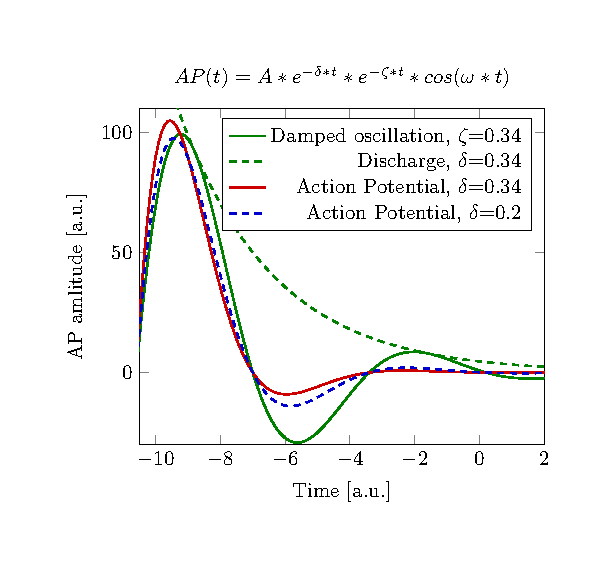
\includegraphics[scale=1.2]{fig/DampedOscillation}
	
	\caption{Describing the generation of an \gls{AP}
		as the superposition of an elastic vibration 
		of the membrane and an electrical discharge process.
		\label{fig:DampedOscillation}}
	
\end{figure}

\else

A $Na^+$ ionok berobbanása a sejtbe elektromos, kémiai és mechanikai grandiens változásokat jelent.
Végeredményként a membrán vibrálni kezd az elektrolitban (lásd~ Fig.~\ref{fig:DampedOscillation} ábra), 
aminek kb. $10^{-3}$-ad része ionizált.  
Ezen felül az ionok taszítása és a koncentrácigradiens 
olyan többlet feszültséget állítanak elő, ami elektromos kisüléshez vezet. A két folyamat egyidejűleg zajlik,
"egymásra ül".

\begin{figure}
\centering
	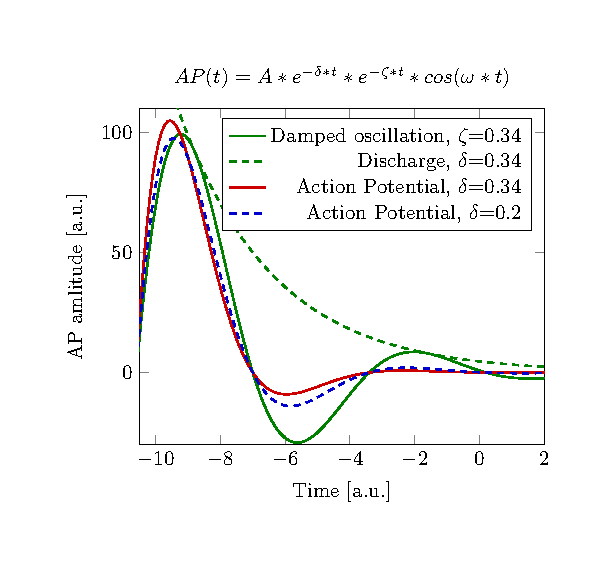
\includegraphics[scale=1.2]{fig/DampedOscillation}
	
	\caption{Az \gls{AP} előállítása egy rugalmas rezgés és egy 
	elektromos kisülés eredőjeként.
		\label{fig:DampedOscillation}}
	
\end{figure}
\fi

\ifx\magyar\undefined
The sudden rush-in of
$Na^+$ ions has (at least) a double effect. 
One effect is that they press the surface of the membrane that
elastically increases its diameter~\cite{NeuronalDeformation:2020}.
Due to their mutual repulsion,
the ions experience a strong electrical force toward the membrane. It represents an impulse $J=F\,\Delta t$ [N\,s], that enables estimating the time and energy of the 
change the rush-in causes and explains that the energy needed to 
generate an \gls{AP} is suddenly produced electrically, 
and stored temporarily as elastic energy (the neuron produces the required energy in the background, when \gls{ATP} produces ions by hydrolysis under the effect of the electrical field near to membrane); see~\cite{VeghUnifiedCrossdisciplinaryModel:2026}. 
The case is practically identical to
the deformation of an elastic plate induced by the hydrostatic pressure of a water column. Initially, the aluminum plate is suddenly subjected to hydrostatic pressure, and it reaches equilibrium after initial oscillations. The diagram line of the process is shown in the figure
\cite{HydrostaticWaterColumn:2021}, and the method of simulation is discussed in \cite{Hydrostatic_SPHinXsys:2021}. Compare the diagram line to the
gradient in Fig.~\ref{fig:PhysicalProcessesMembrane}, middle inset.

\else

A membránba hirtelen beömlő $Na^+$ ionoknak (legalább)
két hatása van.
Az egyik, hogy az erős elektrosztatikus taszítás miatt nyomják a
membrán rugalmas felületét, aminek következtében annak
megnövekszik az átmérője.
Ez egy $J=F\,\Delta t$ [N\,s] erőlökést jelent,
ami megmagyarázza, hogy az \gls{AP} generálásához szükséges
energát az ionok elektrosztatikus taszítása generálja,
ami energia a membrán rugalmas energiájává alakul.
Az erőlökés értelmezése lehetővé teszi a beömlés időtartamámak és energiaváltozásának megbecslését.
(Az energiát a neuron háttérfolyamatok során termeli,
a membrán közeli nagy elektromos erőtér hatására, \gls{ATP};
lásd~\cite{VeghUnifiedCrossdisciplinaryModel:2026}. 
Az effektus azzal azonos módon írható le, hogy egy vízoszlop
hidrosztatikus nyomást fejt ki egy rugalmas fenéklemezre.
Kezdetben az alumíniumlemezt hidrosztatikus nyomásnak tesszük ki, majd oszcillációk után egyensúlyi állapotot ér el.
A nyomáshullámot leíró diagramot a~\cite{HydrostaticWaterColumn:2021} ábra mutatja; a szimulációs módszert~\cite{Hydrostatic_SPHinXsys:2021} tárgyalja. 
Hasonlítsuk össze a diagram alakját a~\ref{fig:PhysicalProcessesMembrane} ábra középsőbetét ábrájával.

\fi

\ifx\magyar\undefined

\physicspanel{phys:ElasticForce}
{The elastic force in neurons}
{
The elastic force is described by the  
\[
F(t) = F_{max}^{elastic}\times e^{-\zeta*t}\times cos(\omega\times t)
\]
\noindent 
formula. The classical model entirely neglects this elastic gradient. However, it is almost four orders of magnitude higher than the electrical and thermodynamic gradients (see Appendix~\ref{sec:Forces}), explaining why the damped elastic oscillation almost perfectly describes 
the time course of the \gls{AP}. However, the elastic force oscillates and decays exponentially, so the dominance of 
the elastic term changes with time.
The electrical model can perfectly describe \gls{AP} since 
the pressure and the electric field are proportional to the number of ions inside a volume.

The other effect is that a large amount of positive charges
appears in the neuron, significantly increasing the membrane's potential. The axon remains on the resting potential, so the potential gradient drives a current.
A discharge process takes place where the amount of charge
inside the neuron exponentially decreases 
\[
F_{electric}(t) = F^{max}_{electric}\times e^{-\delta*t}
\]

The two effects act at the same time, that is
\[
F_{resulting}(t) = F^{max}_{resulting}\times e^{-\delta*t}  \times e^{-\zeta*t}  \times cos(\omega\times t)
\]
(the two exponential factors have physically different reasons,
but they can be contracted mathematically), resulting
an oscillation shown in Fig.~\ref{fig:DampedOscillation}.
This model combines the effects of two distinct disciplines,
but may not be perfect, because of the dual role of ions:
the electric effect changes the oscillating mass and the oscillation changes the amount of charge. However, it 
suggests a way to synthesize the two effects, and explain 
a till now unexplained thermodynamical observation.
}

\else

\physicspanel{phys:ElasticForce}
{A neuronra ható rugalmas erő}
{
A rugalmas erőt a
\[
F(t) = F_{max}^{elastic}\times e^{-\zeta*t}\times cos(\omega\times t)
\]
\noindent 
formula írja le. A klasszikus modell teljességgel elhanyagolja ezt a gradientst, bár az csaknem négy nagyságrenddel meghaladja az elektromos és termodinamikai gradienst (lásd Appendix~\ref{sec:Forces}). Ez megmagyarázza, hogy miért írja le
csaknem pontosan az \gls{AP} időlefutását.
A rugalmas erő azonban oszcillál és exponenciálisan gyengül,
így a rugalmas tag dominanciája időben változik.
Az elektromos modell azért írja le nagyon jól az \gls{AP}-t,
mert az elektromos tér és a nyomás egyaránt az adott térfogatban
levő ionok számával arányos.

A másik hatás, hogy nagy mennyiségű pozitív töltés jelenik meg
a neuronban, ami jelentősen megnöveli a membrán potenciált.
Az axon ekkor még a nyugalmi potenciálon van, 
így a potenciálkülönbség áramot generál.
Kisülési folyamat kezdődik, anelyben a neuronban levő
töltés mennyisége az
\[
F_{electric}(t) = F^{max}_{electric}\times e^{-\delta*t}
\]
\noindent
összefüggésnek megfelelően csökken. Ez a két hatás
egyidejűleg érvényesül, azaz
\[
F_{resulting}(t) = F^{max}_{resulting}\times e^{-\delta*t}  \times e^{-\zeta*t}  \times cos(\omega\times t)
\]
(A két exponenciális tényező fizikai oka ugyan különböző,
de matematikailag összevonhatók).
A modell végeredményben a \ref{fig:DampedOscillation}~ábrán
mutatott oszcillációt eredményezi.

Ez a modell ugyan különböző tudományterületeket kombinál,
de -- az ionok kettős szerepe miatt -- nem lehet tökéletes:
az elektromos töltés változtatja a rezgő tömeget és
a rezgés változtatja a töltés mennyiségét.
Ráirányítja azonban figyelmünket arra, hogy a két 
tudományterület összevonható, és megmagyarázza az eddig
nem értett termodinamikai megfigyelést.
}

\fi


Furthermore, the  elastic model explains the experienced constant intensity
of \gls{AP} (without the ad-hoc hypothesis of cooperating
ion channels in the axon's wall). The vibrating electrolyte 
behaves as a 'soliton'~\cite{SolitonPropagation:2005}, that is, transfers the pressure wave with a minimum material transport and intensity loss, and the dissociated ions inside the vibrated electrolyte generate the potential field observed as \gls{AP}.


\proconpanel
{Elastic/electric neuron model}
{
\begin{itemize}[noitemsep]
	\item Connects mechanical and electrical phenomena
	\item Simple function form to calculate
\end{itemize}
}
{
\begin{itemize}[noitemsep]
	\item Uses empirical coupling factor between disciplines
	\item Not a faithful form
\end{itemize}
}
